\section{Consensus Architecture Context}

\label{sec:architecture}

FPC operates within Lux's physics-inspired consensus architecture, which uses a wave-based metaphor to organize consensus primitives:

\begin{figure}[h]
\centering
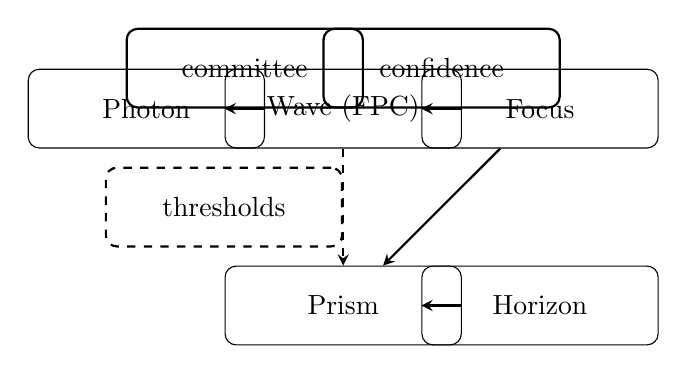
\begin{tikzpicture}[
    node distance=2.5cm,
    every node/.style={draw, rounded corners, minimum width=3cm, minimum height=1cm},
    arrow/.style={->, >=stealth, thick}
]
    \node (photon) {Photon};
    \node (wave) [right of=photon] {Wave (FPC)};
    \node (focus) [right of=wave] {Focus};
    \node (prism) [below of=wave] {Prism};
    \node (horizon) [right of=prism] {Horizon};
    
    \draw[arrow] (photon) -- node[above] {committee} (wave);
    \draw[arrow] (wave) -- node[above] {confidence} (focus);
    \draw[arrow] (focus) -- (prism);
    \draw[arrow] (prism) -- (horizon);
    \draw[arrow, dashed] (wave) -- node[left] {thresholds} (prism);
\end{tikzpicture}
\caption{FPC within the Lux consensus stack architecture}
\label{fig:architecture}
\end{figure}

The architecture follows an optics metaphor where:
\begin{itemize}
\item \textbf{Photon}: Atomic unit that selects $k$ ``rays'' (committee sample)
\item \textbf{Wave}: Per-round thresholds $(\alpha_{\text{pref}}, \alpha_{\text{conf}})$ with phase shifts (FPC layer)
\item \textbf{Focus}: $\beta$ consecutive rounds concentrate confidence into a decision
\item \textbf{Prism}: Geometric views of a DAG (frontiers, cuts, refractions)
\item \textbf{Horizon}: Order-theoretic structure (reachability, antichains, certificates)
\end{itemize}

FPC implements the ``Wave'' layer, providing adaptive thresholds that guide opinion formation through interference patterns analogous to wave physics.

